% Created 2022-09-02 Fri 13:30
% Intended LaTeX compiler: pdflatex
\documentclass[10pt]{beamer}
\usepackage[utf8]{inputenc}
\usepackage[T1]{fontenc}
\usepackage{graphicx}
\usepackage{longtable}
\usepackage{wrapfig}
\usepackage{rotating}
\usepackage[normalem]{ulem}
\usepackage{amsmath}
\usepackage{amssymb}
\usepackage{capt-of}
\usepackage{hyperref}
\usepackage{minted}
\usepackage[T1]{fontenc}
\usepackage{pmboxdraw}
\usetheme{Berkeley}
\usefonttheme{professionalfonts}
\usepackage{booktabs}
\definecolor{mycolor}{rgb}{0.54706, 0.13725, 0.26667}
\usecolortheme[named=mycolor]{structure}
\setlength{\parskip}{5pt}
\newcommand{\footnoteframe}[1]{\footnote[frame]{#1}}
\addtobeamertemplate{footnote}{}{\vspace{2ex}}
\usepackage{xcolor}
\definecolor{LightGray}{gray}{0.95}
\setbeamertemplate{caption}[numbered]
\usepackage{amsmath}
\usepackage{fancyvrb}
\DefineVerbatimEnvironment{verbatim}{Verbatim}{fontsize=\scriptsize}
\DeclareGraphicsRule{.gif}{png}{.png}{`convert #1 `dirname #1`/`basename #1 .gif`-gif-converted-to.png}
\DeclareGraphicsExtensions{.gif}
\usepackage{animate}
\DeclareGraphicsRule{.gif}{png}{-0.png}{`convert #1 `dirname #1`/`basename #1 .gif`-gif-converted-to.png}
\DeclareGraphicsExtensions{.gif}
\usepackage{amsmath}
\author{Jay Morgan}
\date{<TODO>}
\title{Machine Learning\\\medskip
\large Lecture 2 - Linear Models}
\hypersetup{
 pdfauthor={Jay Morgan},
 pdftitle={Machine Learning},
 pdfkeywords={},
 pdfsubject={},
 pdfcreator={Emacs 28.1 (Org mode 9.5.4)}, 
 pdflang={English}}
\begin{document}

\maketitle

\section*{Linear Regression}
\label{sec:org1aed3a6}

\subsection*{Introduction to linear models}
\label{sec:orgc4a2c3c}

\subsubsection*{Linear models}
\label{sec:orgf1c3017}

Having learnt a little about what it means to learn, we're going to look at our first
\emph{Machine Learning} algorithm, the staple for much of statistics, numeric prediction
using a linear model.

\subsubsection*{What is a linear model?}
\label{sec:org787f595}
A linear model is a prediction (a response) to an input variable. We have the
following terms:

\begin{itemize}
\item Response/prediction -- the output of the model.
\item Dependant variable -- the variable upon which the prediction is being made.
\end{itemize}

For a linear model based on one dependant we have the following:

\[
y = w x + b
\]

where \(y\) is the response/output/prediction of the model, \(x\) is the dependant
variable, and \(w, b\) are the model parameters.

\subsubsection*{Slope \& intercept}
\label{sec:org0768375}
If we look at our linear model equation, we'll notice that it's the same equation for a straight line.

\begin{center}
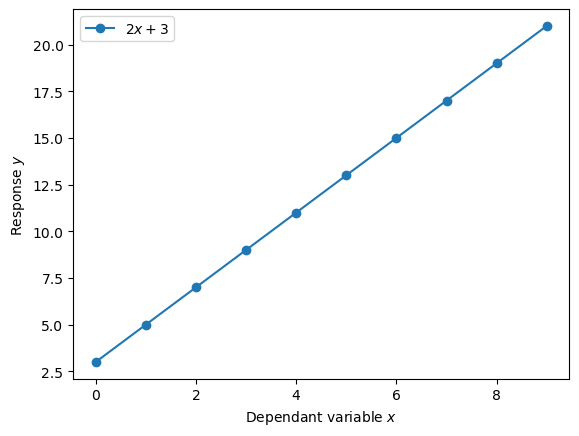
\includegraphics[width=0.5\textwidth]{images/linear_model.png}
\end{center}

As we've seen, the linear model, or linear regression, has two parameters: \(w,
b\). What do these parameters represent?

\begin{itemize}
\item The \(w\) parameter is the \textbf{slope} or strength of relationship between the dependant
variable and the response.
\item Meanwhile, the \(b\) parameter is called the \textbf{intercept}, as it's the value of the
response when the dependant variable is zero.
\end{itemize}

Let's look at these two parameters.

\begin{center}
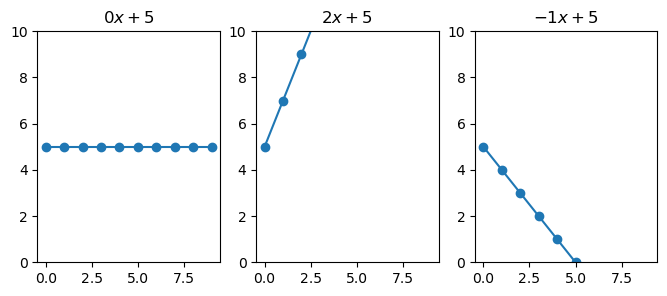
\includegraphics[width=.9\linewidth]{images/slope_1.png}
\end{center}

Here we see that when \(w\) is 0 (left figure), any change in \(x\) results in 0 change
in \(y\). While, with \(w = 2\), \(y\) increases two-fold by every change in \(x\). Finally,
when the slope is negative, we see that \(y\) decreases.

Notice how the line is at 5 when \(x\) is zero, this is because \(b = 5\).

\subsubsection*{Supporting example}
\label{sec:orgf27f81d}

Let's have a look at how we would use this linear model with one of the datasets: The
Boston housing prices.

\begin{figure}[htbp]
\centering
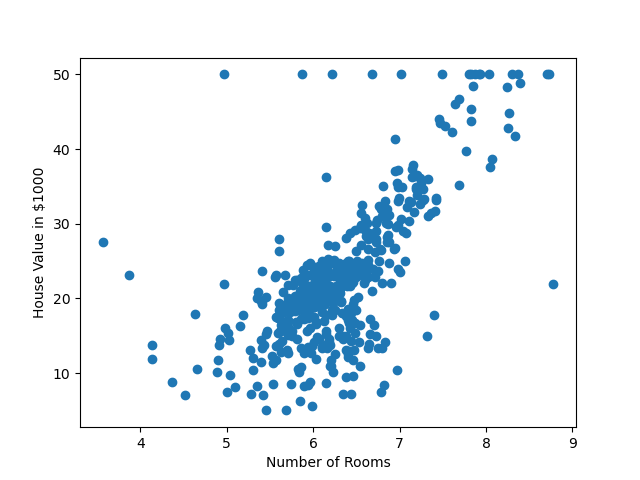
\includegraphics[width=0.6\textwidth]{images/boston_rooms_prices.png}
\caption{Scatter plot of the number of rooms in a house against the house valuation. In this plot we can see a positive effect with some outliers to this trend.}
\end{figure}

\subsubsection*{Let's fit a linear model}
\label{sec:org03224b2}
We have seen that there seems to be some correlation between the number of rooms and
the house price. I.e. we can use the number of rooms of the house to get the
estimated price. To get an estimated price we'll use our linear model:

\[
y = w x + b
\]

In this case, \(x\) will be the number of rooms. But what values should we set for \(w\)
and \(b\)? Or put another way, what is \emph{optimal} value for our model parameters.

We'll return to the question of optimal later, but for now, let's just select some
random values!

\[\begin{aligned}
w = 1 \\
b = 1
\end{aligned}\]


\begin{figure}[htbp]
\centering
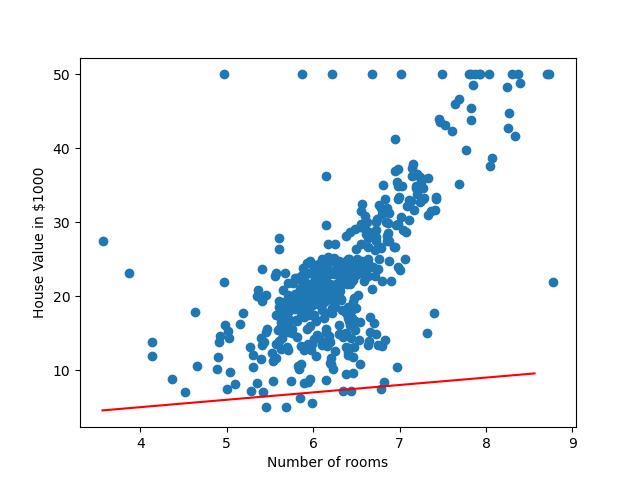
\includegraphics[width=0.6\textwidth]{images/boston_rm_first_pred.png}
\caption{A linear model line overlayed onto the boston house prices dataset. Blue circles represent samples from the dataset, while the trend line is shown in red.}
\end{figure}

Well that doesn't look very good, it could be 'fit' better to what we're seeing in
the scatter plot! I wonder how wrong the linear model is -- how incorrect our
predicted house prices are?

\subsubsection*{Evaluating our initial linear model}
\label{sec:org8d7e59c}
To evaluate how well, or in this case, how badly our linear model is doing, let's
compare the predicted value from the model against the actual house price. For
example, we'll take a single sample from our dataset.

If we have 4 rooms, our model estimates the house price to be \(2(4) + 5 = 13\),
\$13,000, but the actual cost was \$24,000. This means we have underestimated the cost
by \$11,000.

What we've done there is the following:

\[
\delta = | y - \hat{y} |
\]

where \(\hat{y}\) is \(w x + b\)

We've calculated the difference or delta between the real house price \(y\) and the
predicted house price.

That gives us the error for one sample though, what about for the whole dataset? Well
we could take the mean over all samples:

\[
\Delta = \sum_{i=0}^n | y - \hat{y} |
\]

If we calculate that our linear model we see that the average difference between our
estimated value and real value is \$15,000!

\subsubsection*{Getting better model parameters}
\label{sec:orgc134c1d}
Okay, so we made our initial guess at the model parameters (random values for \(w,
b\)), and these weren't very good. We were incorrectly guessing the house value by
\$15,000. So how do we get better values?

Well if we visualise how badly we do vs the value for \(w\) we get the following:

\begin{figure}[htbp]
\centering
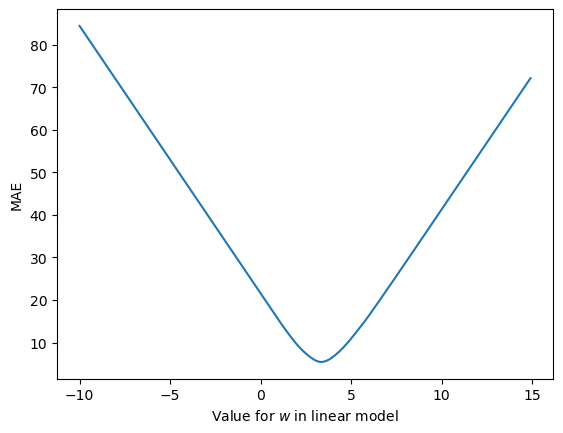
\includegraphics[width=0.6\textwidth]{images/plot_linear_model_loss_w.png}
\caption{\label{fig:mae_lm}Mean absolute error (MAE) between the true and predicted house values when varying the value for \(w\) parameter in the linear model.}
\end{figure}

In figure \ref{fig:mae_lm}, we see that as we change the \(w\) parameter, the mean absolute
error (MAE), i.e. the average difference between the predicted house prices and the
true house prices, changes. Ideally, we would like the error or \textbf{loss} to be as low as
possible. In this case, when \(b = 1\) the lowest possible loss we can hope to achieve
with the linear model is \textasciitilde{} \$5,500.

But what value for \(w\) gets us this lowest value for the loss? Looking at the graph,
we see that the lowest point on the loss curve is somewhere between 0 and 5. Maybe
even 4? While we could look at the curve and pick these parameter values, we're going
to use a better method -- one that give us an optimal value for this loss curve
automatically.

We're going to look at the method called \textbf{Gradient Descent}.

If we visualise our loss curve again, and visualise where \(w = 1\) is on this curve,
we will see:

\begin{center}
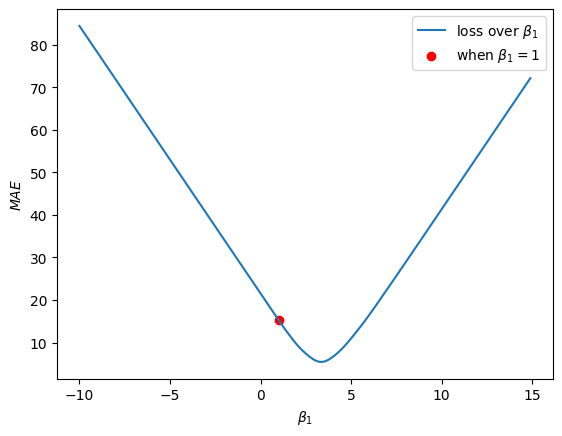
\includegraphics[width=.9\linewidth]{images/loss_curve_w_1.png}
\end{center}

So we want this rot dot to move down the loss curve and reach the bottom of the
curve. Using the \textbf{Gradient Descent} algorithm, we're going to take \textbf{very small steps}
down the loss curve.

\begin{center}
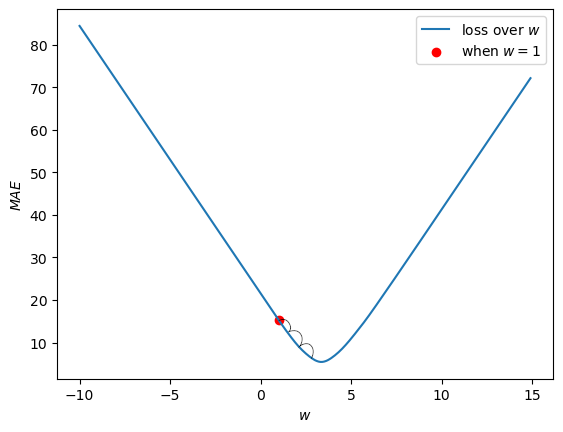
\includegraphics[width=0.6\textwidth]{images/loss_curve_w_1_with_path.png}
\end{center}

To determine which way is up, and which way is down the curve, we use the \textbf{Gradient} of
the curve (hence Gradient Descent). We compute the gradient using finite differences method:

\[
\Delta = \frac{f(x+h) - f(x)}{h}
\]

where \(f(x)\) is the loss when \(w\) takes on the value of \(x\). \(h\) is a very small
value.

\begin{center}
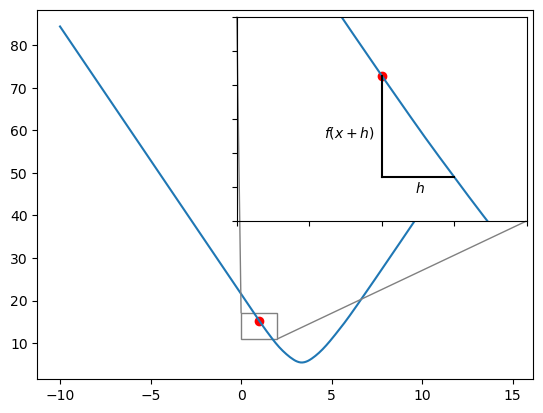
\includegraphics[width=.9\linewidth]{images/small_step.png}
\end{center}

If we select \(h = 0.5\) then we will have the formula:

\[
\Delta_w = \frac{\mathcal{L}(w + 0.5) - \mathcal{L}(w)}{w}
\]

where \(\mathcal{L}\) represents our loss function, MAE. If we calculate this we have:
\[\begin{aligned}
\Delta_w &= \frac{\mathcal{L}(w + 0.5) - \mathcal{L}(w)}{h} \\
&= \frac{\mathcal{L}(1.5)- \mathcal{L}(1)}{1  - (0.5)} \\
&= \frac{12 - 15}{0.5} \\
&= -6.0
\end{aligned}\]

Given that the gradient is a negative number, we know that the curve is going
down/decreasing. So we will want to move \(w\) in this direction -- we want to move
\(w\) so that the loss decreases.

\[
\overline{w} = w - \eta \Delta_w
\]

If we plug in the numbers we've calculated for when \(w = 1\) we get and \(eta = 0.5\):

\[\begin{aligned}
\overline{w} &= w - \eta \Delta_w \\
&= 1.0 - (0.5 * -6.0) \\
&= 1.0 - (-3.0) \\
&= 4.0
\end{aligned}\]

Our new value for the \(w\) parameter (\(\overline{w}\)) is computed by taking its
original value and subtracting the gradient modulated/multiplied by \(\eta\). \(\eta\) in
this case is what will allow us to take our \textbf{small steps}. It is important to set
\(\eta\) to a suitably small value, as high values for \(\eta\) will cause the Gradient
Descent to behave erratically, and even, make our loss worse!

\begin{figure}[htbp]
\centering
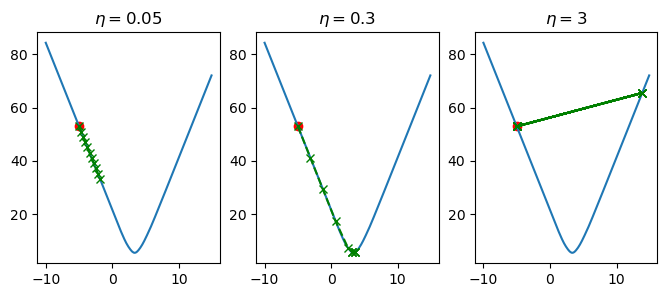
\includegraphics[width=.9\linewidth]{images/small_step_eta.png}
\caption{\label{fig:eta}Plotting the effect of \(\eta\) on the step change of \(w\).}
\end{figure}

In figure \ref{fig:eta}, we've varied the value of \(\eta\) and computed 10 steps of updating
the \(w\) parameter in our linear model. When \(\eta=0.05\), we see that \(w\) is slowly
being updated in a way that is causing our loss to decrease, but it is more so slowly
that we don't reach the optimal value for \(w\). When \(\eta=3\), each change in \(w\) is
too large, so we over-shoot the optimal value, and end up bouncing back and forth
without ever improving. Finally, when we set \(\eta=0.3\), the changes in \(w\) are
sufficiently large enough such that we reach the \textbf{global minima} in time, but they are
also small enough so that we don't over-shoot this same minimum.

If we then apply the Gradient Descent algorithm to both parameters of the linear
model \(w, b\), then we can find the optimal trend line for this data. Furthermore,
visualising this will look something like figure \ref{fig:lm_learn}.

\begin{figure}[htbp]
\centering
\includegraphics[width=0.5\textwidth]{images/lm_learn.gif}
\caption{\label{fig:lm_learn}Visualising (GIF) the linear model as its parameters improve.}
\end{figure}


\subsubsection*{Multiple variables}
\label{sec:orgf24f01d}

\section*{Logistic Regression}
\label{sec:orgcc4ced2}

\subsection*{Classification}
\label{sec:org584b67d}

\subsubsection*{Moving from regression to classification}
\label{sec:org8f320bd}

We now turn to classification
\end{document}
